%pour la mise en page
\documentclass[a4paper,12pt]{report}
\usepackage[utf8]{inputenc}
\usepackage{indentfirst}

%pour les figures
\usepackage{float}
\usepackage{graphicx}

%pour les maths
\usepackage{amsmath}
\usepackage{amsfonts}

%pour les hyperliens
\usepackage{hyperref}
\usepackage{url}
\def\UrlBreaks{\do\/\do-}

\usepackage[top=3cm, bottom=3cm, left=3cm, right=3cm]{geometry}

\usepackage{fancyhdr}
\pagestyle{fancy}
\renewcommand\headrulewidth{1pt}
\fancyhead[L]{Rapport de projet - INF8225}
\fancyhead[R]{}
\renewcommand\footrulewidth{1pt}
\fancyfoot[L]{}
\fancyfoot[C]{\thepage}
\fancyfoot[R]{}

\makeatletter
\let\ps@plain=\ps@fancy
\renewcommand{\thesection}{\@arabic\c@section.}
\renewcommand{\thesubsection}{\@arabic\c@section.\@arabic\c@subsection}
\renewcommand{\bibname}{Bibliographie}
\makeatother

\begin{document}
\begin{titlepage}

  \begin{center}
  \vspace*{4cm}
    \rule{\linewidth}{0.5pt}
    \bigbreak
    {\Huge {INF8225} }
    \bigbreak
    {\LARGE {Rapport de projet}}
    \medbreak    
    \rule{\linewidth}{.5pt}
    \bigbreak
    Michel Fabrice \textsc{Serret}\\
    Justine \textsc{Marlow}\\
    Brieuc \textsc{Dandin}\\
    Nicolas \textsc{Valenchon}\\
    \vfill
	
\includegraphics[scale=1]{Logo_Polytechnique_Montréal_(partenariat_Wikimédia).png}
	\vfill
    
\end{center}
\end{titlepage}

\section*{Introduction}
L'objectif de notre projet est d'observer les effets de la combinaison de deux méthodes en apprentissage par renforcement :
\begin{itemize}
    \item l'imitation dans l'apprentissage
    \item l'utilisation de la curiosité dans l'apprentissage
\end{itemize}
En outre, nous souhaitons déterminer si l'utilisation conjointe ou séquentielle de ces deux méthodes permet d'améliorer les performances du modèle au delà des deux méthodes séparées.

\section{Présentation du modèle}
\subsection{Méthode de curiosité choisie}
Parmi les méthodes de curiosité qui nous intéressait :
\begin{itemize}
    \item \textit{Curiosity-driven Exploration by Self-supervised Prediction} \cite{curiosity}
    \item \textit{Exploration by Random Network Distillation} \cite{distillation}
    \item les méthodes utilisées par les agents de \textit{Never Give Up} \cite{ngu} et de l'agent 57 \cite{agent57}
\end{itemize}
Nous avons choisi d'utiliser la \textit{random network distillation} en utilisant le code fourni avec l'article de recherche (disponible sur un \textit{repository Github} \cite{distillation_github}). On présentera cette méthode dans la section \ref{revue_distillation} en page \pageref{revue_distillation} de ce rapport.

\subsection{Méthode d'imitation choisie}
Notre objectif était d'utiliser la méthode d'apprentissage par renforcement par imitation \textit{SQIL} \cite{sqil}.\\
\indent Cependant, dû à un manque de temps et le fait de n'avoir trouvé aucun \textit{repository} utilisable, nous avons décidé de définir une récompense intrinsèque guidée par les démonstrations d'un agent expert (ici, notre agent entraîné avec la curiosité de \textit{random network distillation}).\\
\indent Pour ce faire nous avons utilisé une méthode similaire au \textit{pseudo-count} de la mémoire épisodique de l'agent NGU mais pour comparer les observations de notre agent avec celles des démonstrations de notre agent expert. Par manque de temps, et comme nous nous intéressons ici à ce que les états soit similaire nous avons utilisée directement les produit scalaire entre les vecteurs de \textit{features} crées par le \textit{random target network} du modèle en cours d'entraînement comme \textit{kernel} de similarité, ensuite nous combinons le \textit{reward} ainsi obtenu avec le \textit{reward} de curiosité comme suit:
\begin{equation} r_{im} = \frac{\sum_{v\in \text{Demonstrations}} X_{obs}\cdot v}{|\text{Demonstrations}|} \end{equation}

\begin{equation} r_{int} = r_{rnd} \cdot (1 + tanh(\alpha \cdot r_{im})) \end{equation}

\newpage \section{Revue : \textit{Exploration by Random Network Distillation}}
\label{revue_distillation}

\newpage \section{Expériences}
\subsection{Combinaison de l'imitation et de la curiosité}
Nous avons donc choisi de comparer les performances de notre agent avec curiosité (\textit{random network distillation}) avec notre agent imitateur de l'agent \textit{expert} (le premier).
Notre implémentation du reward $r_{im}$, défini ci-dessus, souffre d'une erreur dont nous n'avons malheureusement pas trouvé la source et qui nous empêche d'aller au-delà de 400 étapes par épisode durant l'entrainement.
En effet, l'apprentissage avec ce reward fonctionne jusqu'à ce que la mémoire de l'ordinateur soit remplie et que les process MPI et python associés soient 'killed'.
Malgré la diminution du nombre de processes concurrent à 8(initialement 32) et du nombre d'observations de l'agent expert à 54 (initialement 864), nous n'avons pas pu aller au-delà d'épisodes de 400 étapes pour l'entrainement avec ce reward.
Cette erreur est probablement dûe à un 'memory-leak' dans notre code, cependant l'hypothèse du manque de mémoire n'a pas été écartée(par manque de moyen).

\subsection{Environnement de test}
%Pour tester notre modèle, nous avons utilisé la librairie \textit{python} \textit{gym} \cite{gym}, qui permet de tester et comparer des modèles en apprentissage par renforcement, notamment sur des jeux vidéos.\\
Le code fourni pour la \textit{random network distillation} offre différents environnements de test qui sont des jeux vidéos d'\textit{Atari}, nous avons choisi d'entraîner et de tester nos agents sur le jeu \textit{Montezuma's revenge}\cite{montezuma}. Dans ce jeu, l'objectif du joueur est d'explorer un ensemble de salles en évitant des ennemis et des pièges (qui entraînent la mort du joueur).

\subsection{Résultats}
\subsubsection{Agent avec curiosité (\textit{random network distillation})}
On va s'intéresser à différents paramètres que l'on peut observer au fil de l'apprentissage de l'agent à savoir :
\begin{itemize}
    \item \textit{n\_rooms} : le nombre de salles atteintes par l'agent depuis le début de l'apprentissage
    \item \textit{rewtotal} : la somme des récompenses obtenues par l'agent depuis le début de l'apprentissage
    \item \textit{best\_ret} : la valeur de récompense la plus importante déjà rencontrée par l'agent depuis le début de l'apprentissage
    \item \textit{eplen} : la longueur des épisodes d'apprentissage menés par l'agent
    \item \textit{eprooms} : le nombre de salles atteintes par l'agent en un épisode d'apprentissage
\end{itemize}

\begin{figure}[H]
    \centering
    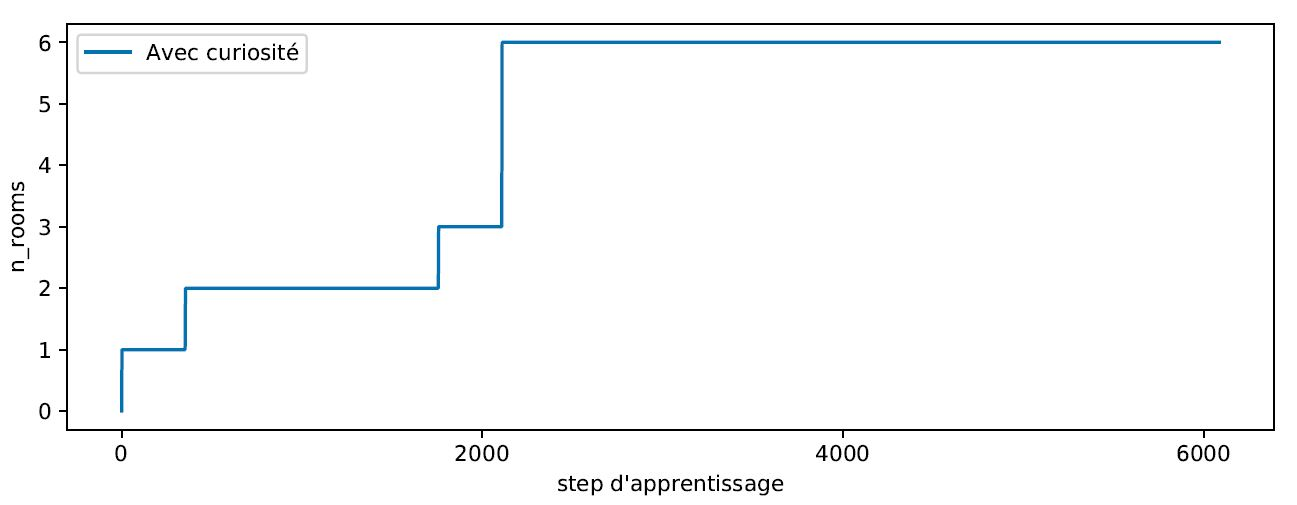
\includegraphics[width=\textwidth]{curiosity_only/curiosity_n_rooms.JPG}\\
    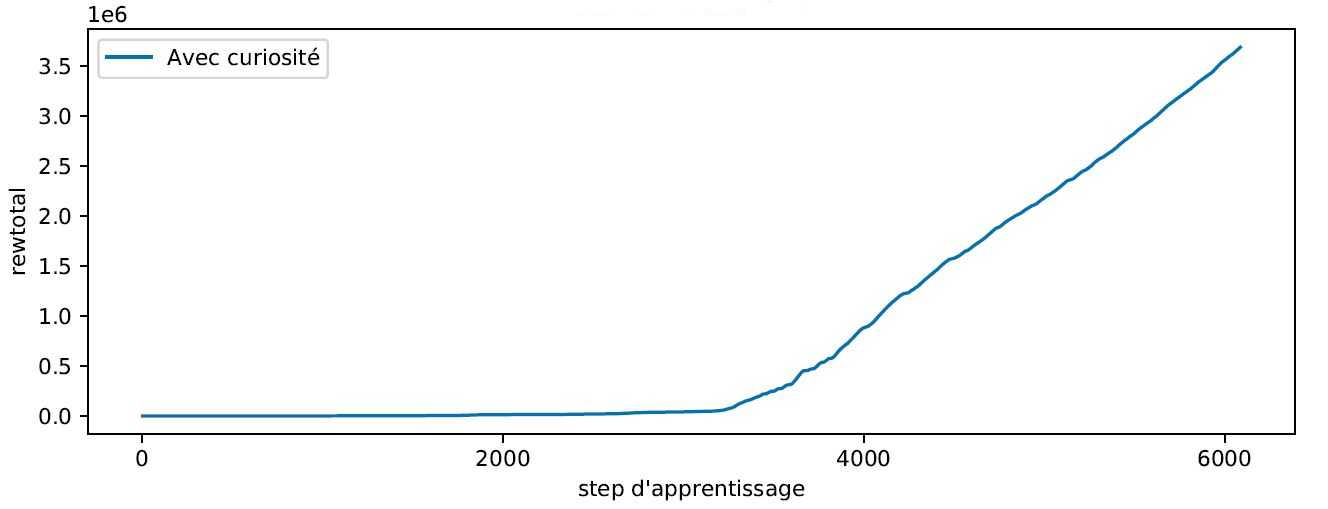
\includegraphics[width=\textwidth]{curiosity_only/curiosity_rewtotal.JPG}\\
    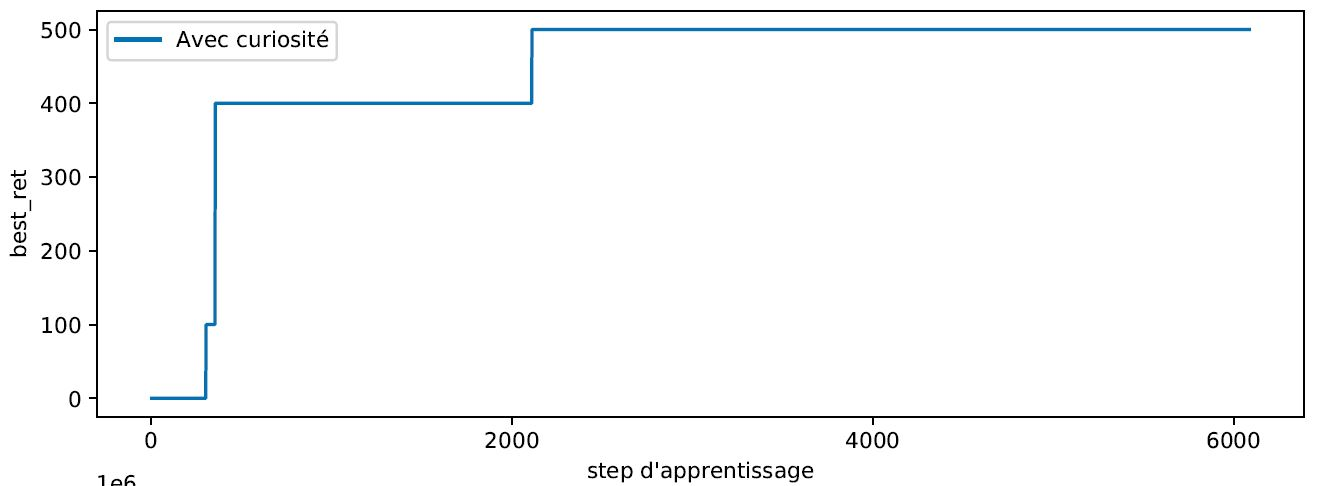
\includegraphics[width=\textwidth]{curiosity_only/curiosity_best_ret.JPG}
    \caption{Résultats de l'apprentissage de l'agent avec curiosité (1)}
\end{figure}

\begin{figure}[H]
    \centering
    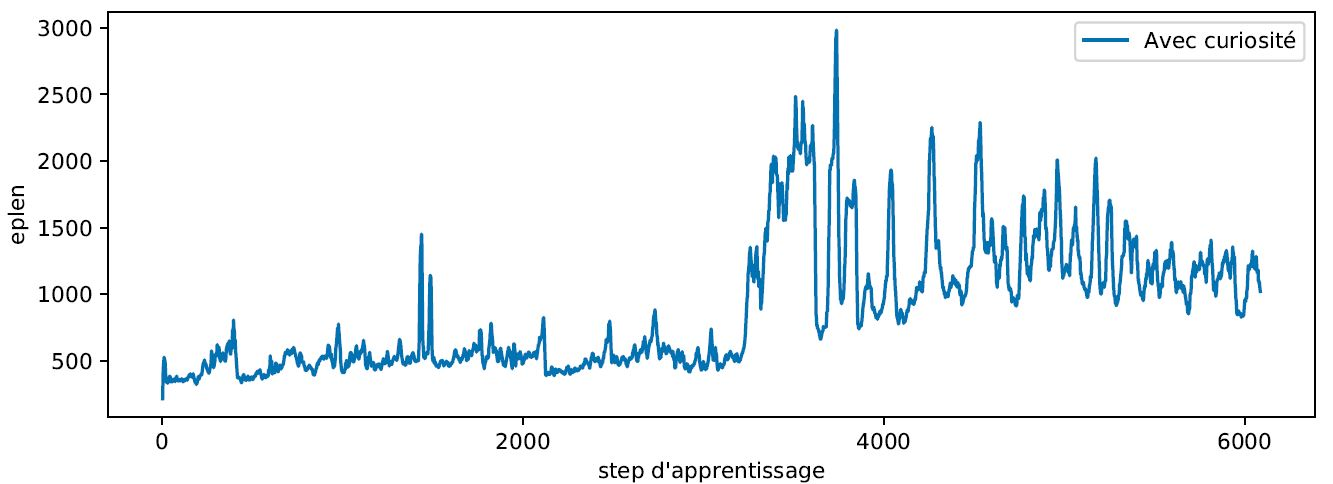
\includegraphics[width=\textwidth]{curiosity_only/curiosity_eplen.JPG}\\
    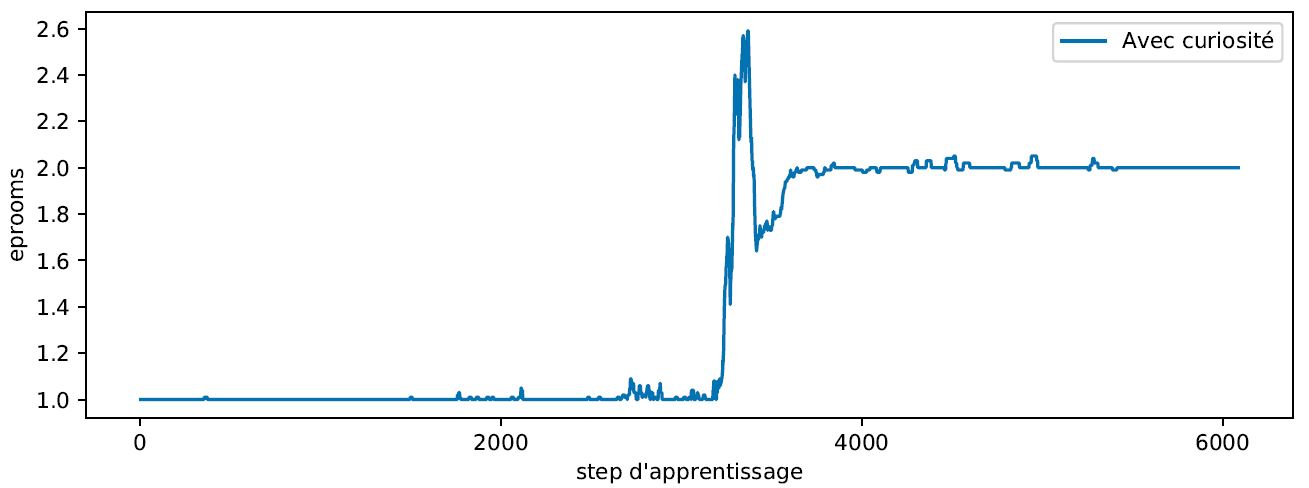
\includegraphics[width=\textwidth]{curiosity_only/curiosity_eprooms.JPG}
    \caption{Résultats de l'apprentissage de l'agent avec curiosité (2)}
\end{figure}

\subsubsection{Agent avec imitation}
\begin{figure}[H]
    \centering
    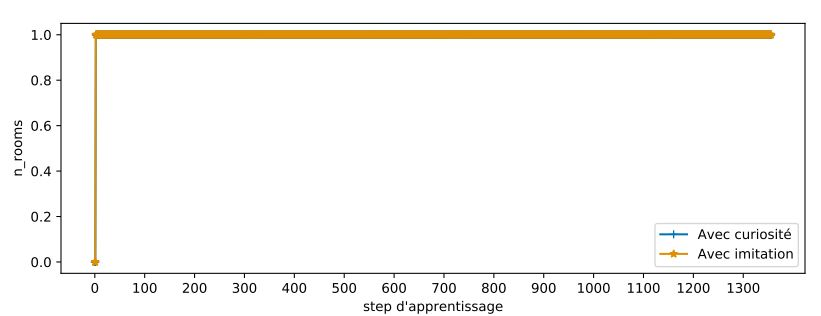
\includegraphics[width=\textwidth]{curiosity_imitation/curiosity_imitation_n_rooms.JPG}
    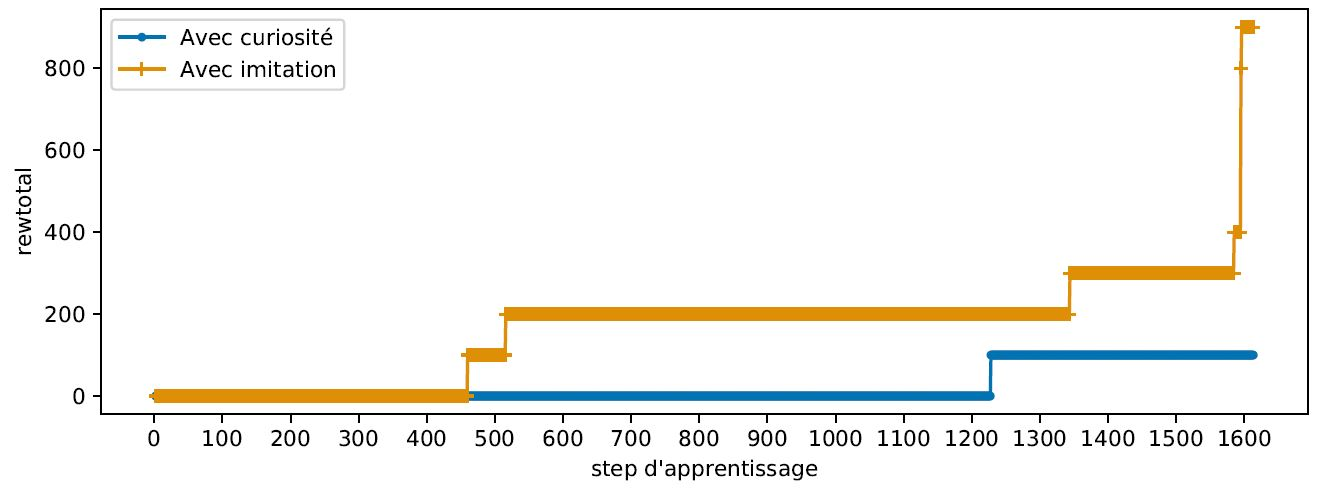
\includegraphics[width=\textwidth]{curiosity_imitation/curiosity_imitation_rewtotal.JPG}
    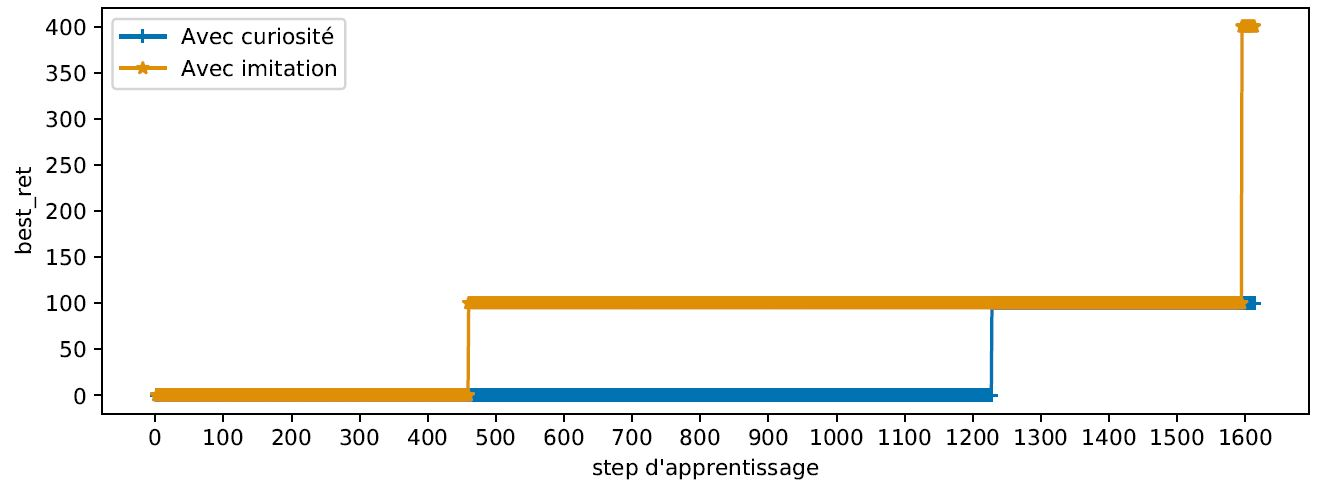
\includegraphics[width=\textwidth]{curiosity_imitation/curiosity_imitation_best_ret.JPG}
    \caption{Comparaison des résultats d'apprentissage de l'agent avec curiosité et de l'agent par imitation (1)}
\end{figure}

\begin{figure}[H]
    \centering
    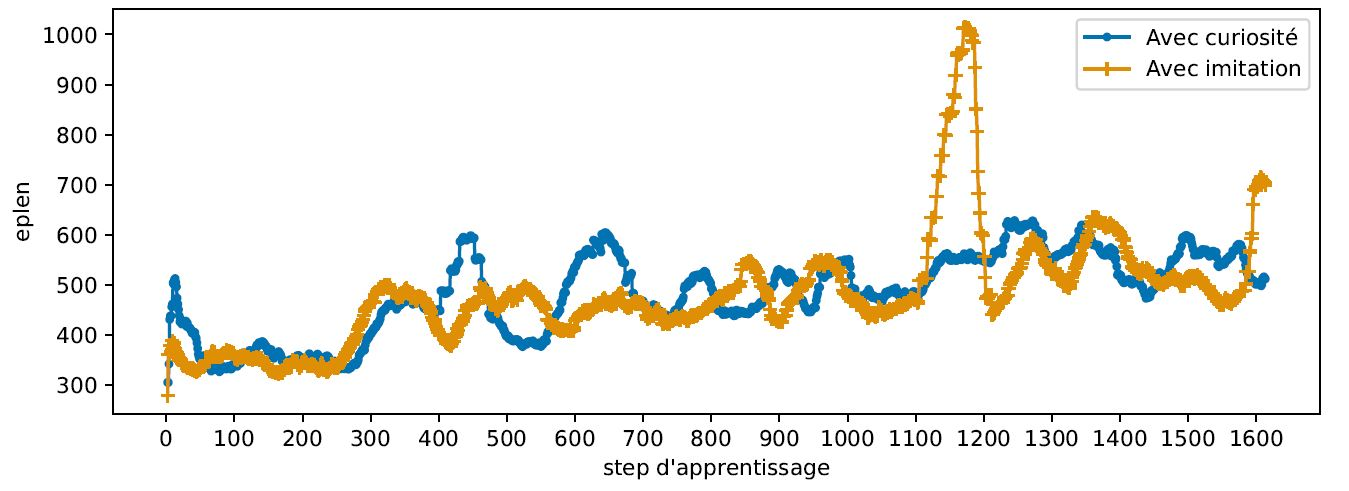
\includegraphics[width=\textwidth]{curiosity_imitation/curiosity_imitation_eplen.JPG}
    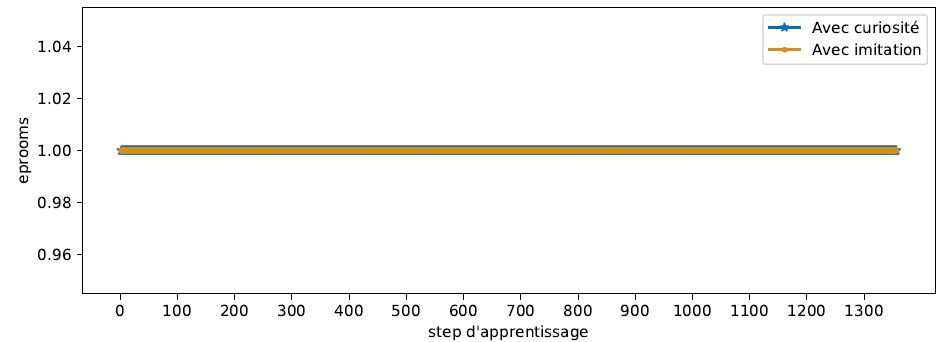
\includegraphics[width=\textwidth]{curiosity_imitation/curiosity_imitation_eprooms.JPG}
    \caption{Comparaison des résultats d'apprentissage de l'agent avec curiosité et de l'agent par imitation (2)}
\end{figure}

\section*{Conclusion}

\begin{thebibliography}{9}
    \bibitem{curiosity}
	  Deepak Pathak, Pulkit Agrawal, Alexei A. Efros, Trevor Darrell,\\
	  \textit{Curiosity-driven Exploration by Self-supervised Prediction},\\
	  Mai 2017,\\
	  \url{https://arxiv.org/abs/1705.05363}
	  
    \bibitem{distillation}
	 Yuri Burda, Harrison Edwards, Amos Storkey, Oleg Klimov,\\
	  \textit{Exploration by Random Network Distillation},\\
	  Octobre 2016,\\
	  \url{https://arxiv.org/abs/1810.12894}
	  
    \bibitem{ngu}
	 Adrià Puigdomènech Badia, Pablo Sprechmann, Alex Vitvitskyi, Daniel Guo, Bilal Piot, Steven Kapturowski, Olivier Tieleman, Martín Arjovsky, Alexander Pritzel, Andew Bolt, Charles Blundell,\\
	  \textit{Never Give Up: Learning Directed Exploration Strategies},\\
	  Février 2020,\\
	  \url{https://arxiv.org/abs/2002.06038}
	  
    \bibitem{agent57}
	 Adrià Puigdomènech Badia, Bilal Piot, Steven Kapturowski, Pablo Sprechmann, Alex Vitvitskyi, Daniel Guo, Charles Blundell,\\
	  \textit{Agent57: Outperforming the Atari Human Benchmark},\\
	  Mars 2020,\\
	  \url{https://arxiv.org/abs/2003.13350}
	  
    \bibitem{distillation_github}
	  \textit{Github repo for random network distillation}\\
	  \url{https://github.com/openai/random-network-distillation}
	  
		\bibitem{sqil}
	  Siddharth Reddy, Anca D. Dragan, Sergey Levine,\\
	  \textit{SQIL: Imitation Learning via Reinforcement Learning with Sparse Rewards},\\
	  Septembre 2019,\\
	  \url{https://arxiv.org/abs/1905.11108}
	  
	\bibitem{gym}
	\textit{Gym python library}\\
	\url{https://gym.openai.com/}
	
	\bibitem{montezuma}
	Jeu vidéo \textit{Montezuma's revenge}\\
	\url{https://en.wikipedia.org/wiki/Montezuma%27s_Revenge_(video_game)}
\end{thebibliography}

\end{document}